\documentclass[10pt,twocolumn,letterpaper]{article}

%%%%%%%%% PAPER TYPE  - PLEASE UPDATE FOR FINAL VERSION
% \usepackage{cvpr}              % To produce the CAMERA-READY version
% \usepackage[review]{cvpr}      % To produce the REVIEW version
\usepackage[pagenumbers]{cvpr} % To force page numbers, e.g. for an arXiv version

% Import additional packages in the preamble file, before hyperref
%
% --- inline annotations
%
\newcommand{\red}[1]{{\color{red}#1}}
\newcommand{\todo}[1]{{\color{red}#1}}
\newcommand{\TODO}[1]{\textbf{\color{red}[TODO: #1]}}
% --- disable by uncommenting  
% \renewcommand{\TODO}[1]{}
% \renewcommand{\todo}[1]{#1}



% It is strongly recommended to use hyperref, especially for the review version.
% hyperref with option pagebackref eases the reviewers' job.
% Please disable hyperref *only* if you encounter grave issues, 
% e.g. with the file validation for the camera-ready version.
%
% If you comment hyperref and then uncomment it, you should delete *.aux before re-running LaTeX.
% (Or just hit 'q' on the first LaTeX run, let it finish, and you should be clear).
\definecolor{cvprblue}{rgb}{0.21,0.49,0.74}
\usepackage[pagebackref,breaklinks,colorlinks,allcolors=cvprblue]{hyperref}

%%%%%%%%% PAPER ID  - PLEASE UPDATE
\def\paperID{10866} % *** Enter the Paper ID here
\def\confName{CVPR}
\def\confYear{2025}

\def\@fnsymbol#1{\ensuremath{\ifcase#1\or *\or \dagger\or \ddagger\or
   \mathsection\or \mathparagraph\or \|\or **\or \dagger\dagger
   \or \ddagger\ddagger \else\@ctrerr\fi}}

%%%%%%%%% TITLE - PLEASE UPDATE
\title{Large Motion Video Autoencoding with Cross-modal Video VAE}
% \title{A Cross-modal Video VAE for Video Autoencoding with Large Motion}
%%%%%%%%% AUTHORS - PLEASE UPDATE
% \author{First Author\\
% Institution1\\
% Institution1 address\\
% {\tt\small firstauthor@i1.org}
\author{Yazhou Xing\thanks{equal contribution}  \quad Yang Fei$^{*}$ \quad Yingqing He$^{*}$\thanks{corresponding authors} \quad Jingye Chen\quad Jiaxin Xie \\ \quad Xiaowei Chi \quad Qifeng Chen$^{\dagger}$
\\
The Hong Kong University of Science and Technology
}
% For a paper whose authors are all at the same institution,
% omit the following lines up until the closing ``}''.
% Additional authors and addresses can be added with ``\and'',
% just like the second author.
% To save space, use either the email address or home page, not both
% \and
% Second Author\\
% Institution2\\
% First line of institution2 address\\
% {\tt\small secondauthor@i2.org}
% }

\begin{document}
\maketitle
\begin{abstract}
Diffusion Models have emerged as powerful generative models for high-quality image synthesis, with many subsequent image editing techniques based on them. However, the ease of text-based image editing introduces significant risks, such as malicious editing for scams or intellectual property infringement. Previous works have attempted to safeguard images from diffusion-based editing by adding imperceptible perturbations. These methods are costly and specifically target prevalent Latent Diffusion Models (LDMs), while Pixel-domain Diffusion Models (PDMs) remain largely unexplored and robust against such attacks. Our work addresses this gap by proposing a novel attacking framework with a feature representation attack loss that exploits vulnerabilities in denoising UNets and a latent optimization strategy to enhance the naturalness of protected images. Extensive experiments demonstrate the effectiveness of our approach in attacking dominant PDM-based editing methods (e.g., SDEdit) while maintaining reasonable protection fidelity and robustness against common defense methods. Additionally, our framework is extensible to LDMs, achieving comparable performance to existing approaches.
\end{abstract}
    
\section{Introduction}
\label{sec:intro}

\begin{figure*}[t]
\centering
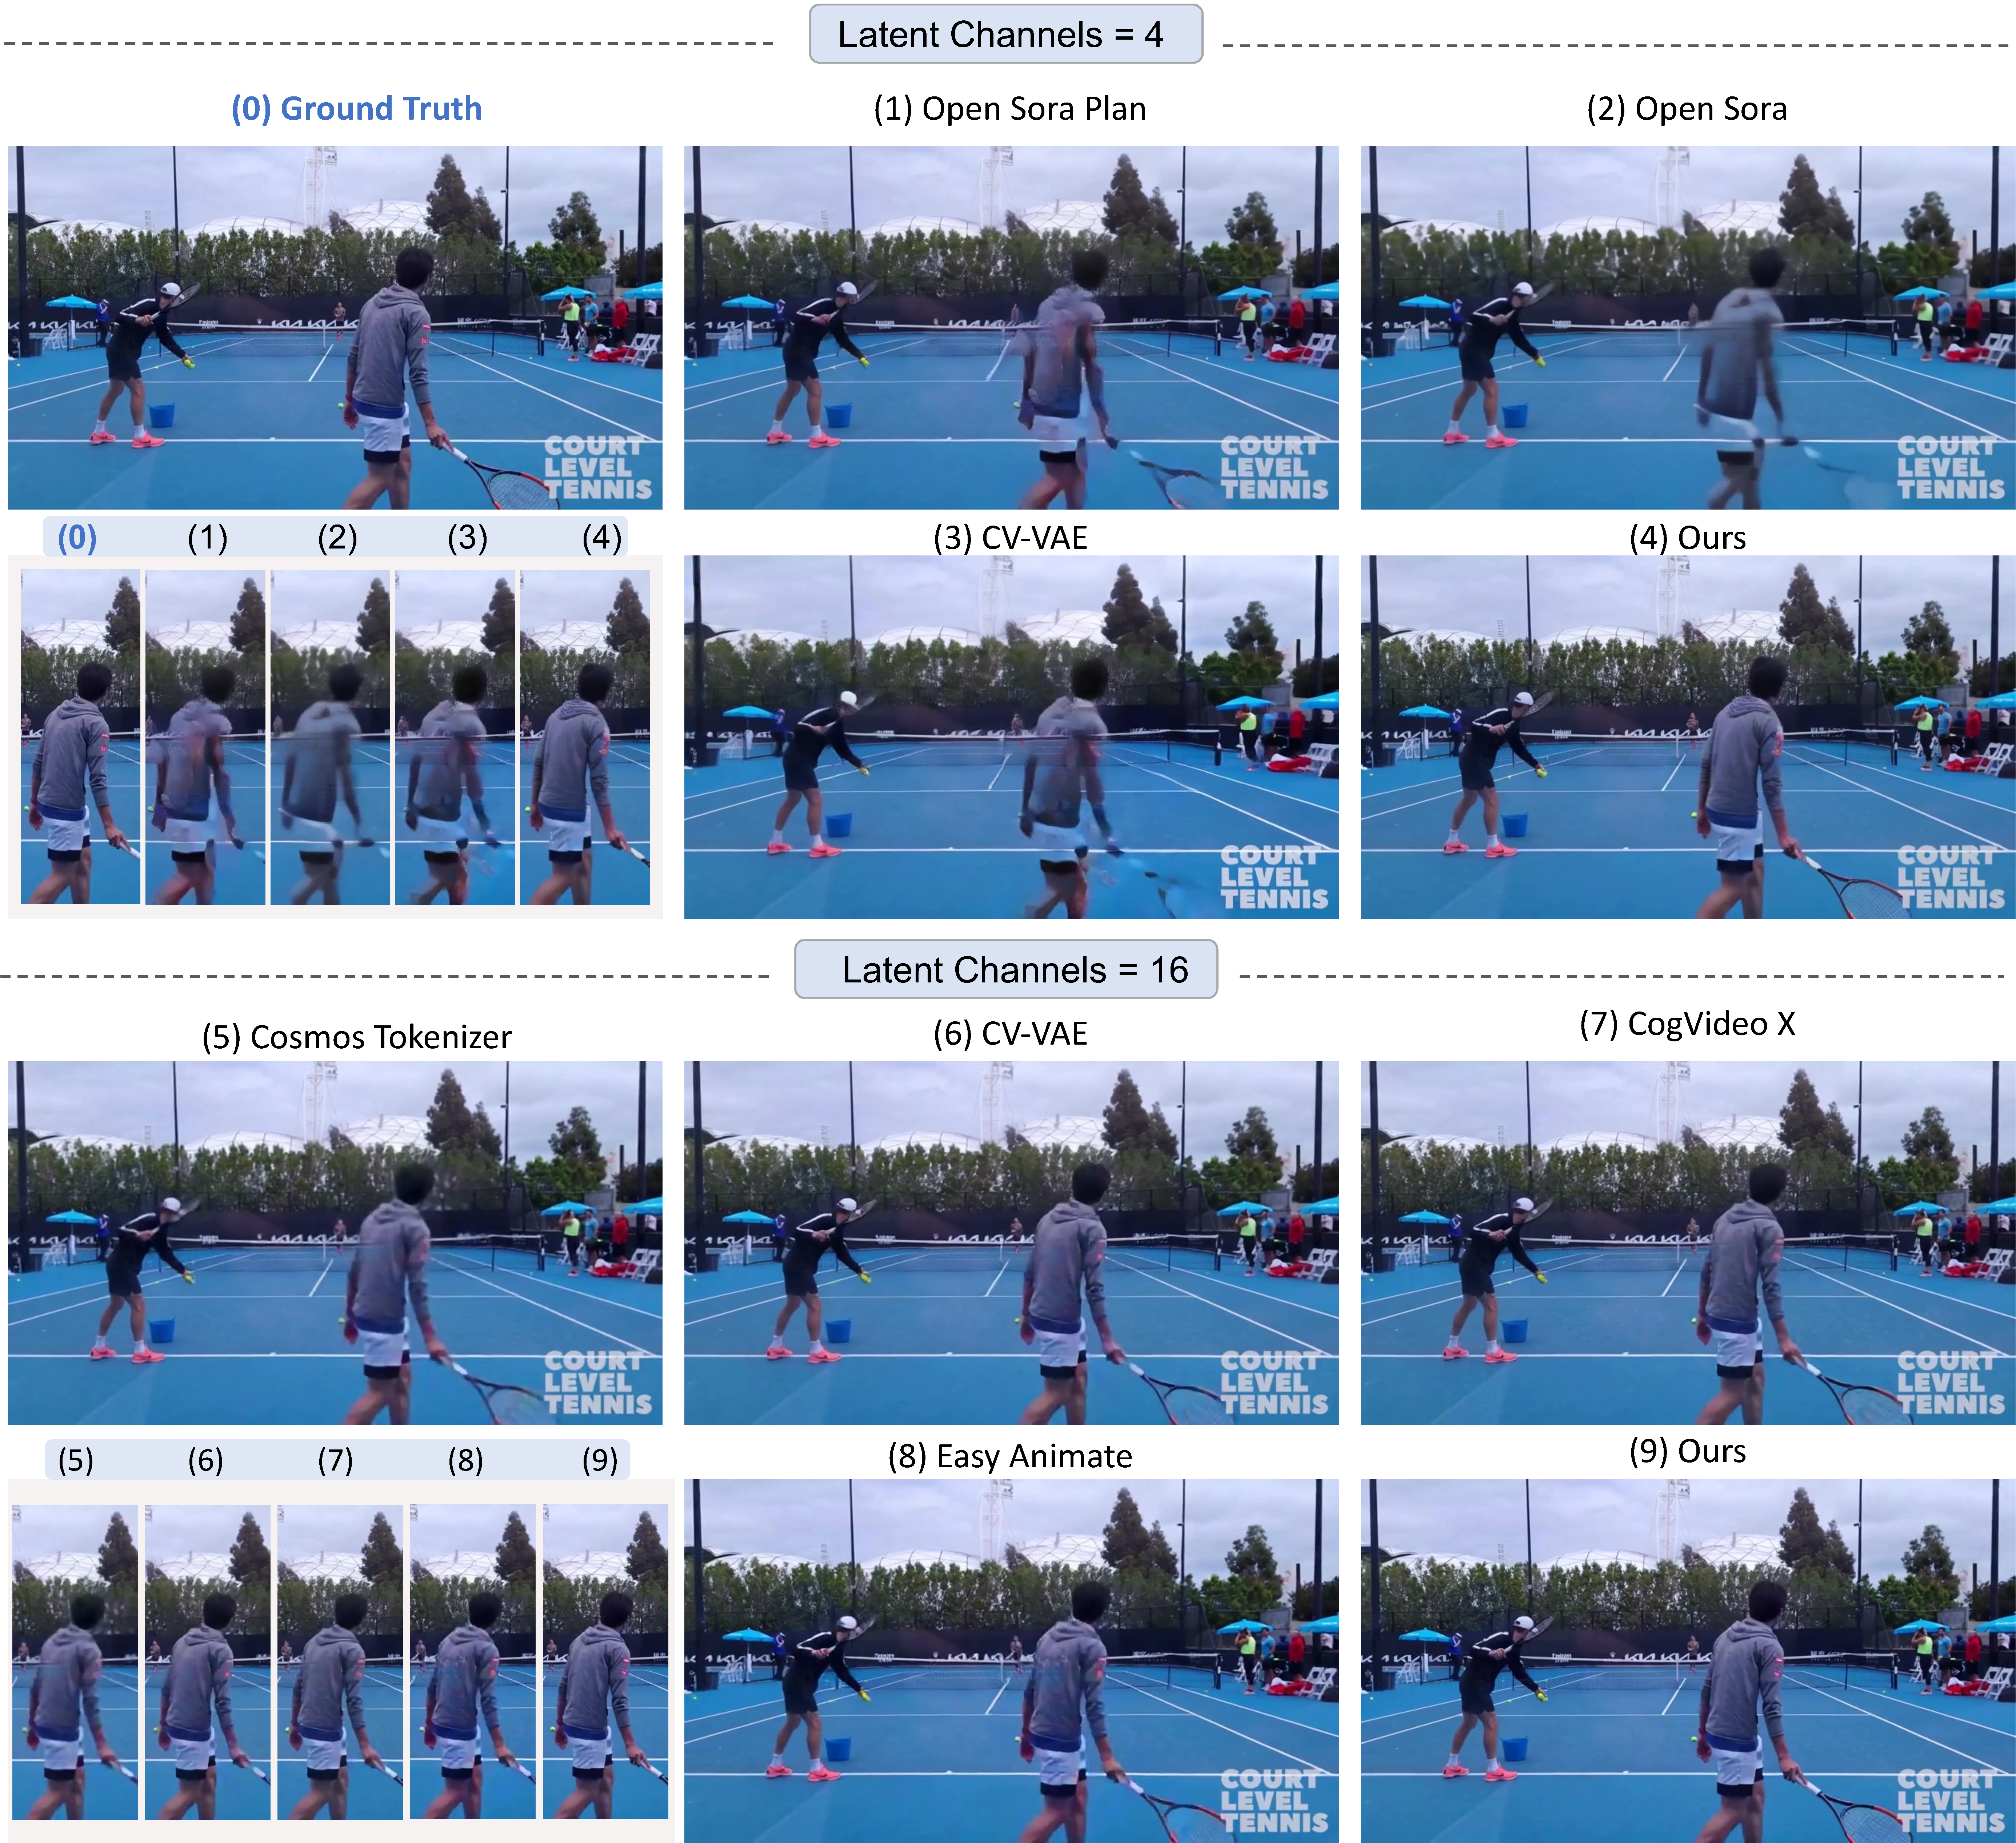
\includegraphics[width=1.0\textwidth]{images/fig1-4and16.pdf}
\caption{
Our reconstruction results compared with a line of three recent strong baseline approaches. 
The ground truth frame is (0). Our model significantly outperforms previous methods, especially under large motion scenarios such as people doing sports.
}
\label{fig:teaser}
\vspace{-3mm}
\end{figure*}



Given the significant attention in the field of video generation, Latent Video Diffusion Models (LVDMs)~\cite{blattmann2023stable, blattmann2023align, he-lvdm, zhou2022magicvideo, he-videocrafter1} have emerged as a popular framework. They have been successfully applied to powerful text-to-video models such as Sora~\cite{videoworldsimulators2024}, VideoCrafter~\cite{he-videocrafter1, chen2024videocrafter2overcomingdatalimitations}, and CogVideoX~\cite{yang2024cogvideox}.
Different from directly generating video pixels, LVDMs generate latent video representations in a compact latent space. This is achieved by first training a Video VAE to encode videos into this latent space.
%
Thus, Video VAE, as a key and fundamental component of LVDMs, has attracted great attention recently.
%
An effective Video VAE can help to reduce the training costs of video diffusion models while improving the final quality of the generated videos.
%
Initially, a series of studies adopt the image VAE from Stable Diffusion~\cite{rombach2022high} for video generation tasks, including AnimateDiff~\cite{guoanimatediff}, MagicVideo~\cite{zhou2022magicvideo}, VideoCrafter1~\cite{he-videocrafter1}, and VideoCrafter2~\cite{chen2024videocrafter2overcomingdatalimitations}. 
%
However, directly adopting an image VAE and compressing video on a frame-by-frame basis leads to temporal flickering due to the lack of temporal correlation. Additionally, the information redundancy along the temporal dimension is not reduced, leading to low training efficiency for subsequent latent video diffusion models.
%
From the introduction of Sora, which compresses videos both temporally and spatially through a Video VAE, a series of studies have emerged that aim to replicate Sora and train their own Video VAEs, including Open Sora~\cite{opensora}, Open Sora Plan~\cite{pku_yuan_lab_and_tuzhan_ai_etc_2024_10948109}, CV-VAE~\cite{zhao2024cv}, CogVideoX~\cite{yang2024cogvideox}, EasyAnimate~\cite{xu2024easyanimatehighperformancelongvideo}, and Cosmos Tokenizer~\cite{cosmos_token}.
%
However, the performance of the current video VAE suffers from many problems, including motion ghost, low-level temporal flickering, blurring (faces, hands, edges, texts), and motion stuttering (lack of correct temporal transition).
% as shown in Fig.~\ref{fig:teaser}.


In this work, we propose a novel cross-modal Video VAE with better spatial and temporal modeling ability in order to solve the aforementioned challenge problems and obtain a robust and high-quality Video VAE.
%
First, we examine different designs for spatial and temporal compression, including simultaneous spatial-temporal (ST) compression and sequential ST compression. 
%
We observed that simultaneous ST compression achieves better low-level temporal smoothness and texture stability, while sequential ST compression achieves better motion recovery, particularly in scenarios of large motion.
%
Thus, we propose a novel architecture that integrates the advantages of both methods and enables effective video detail and motion reconstruction.

Second, we observed that the normally used datasets for text-to-video generation contain text-video pairs. 
Also, during decoding, a text description exists as it serves as the input in the first stage, \textit{i.e.}, the video latent generation stage.
%
To this end, we integrate the text information into the encoding and decoding procedure and propose the first Cross-modal Video VAE.
%
We carefully study how text guidance can be integrated into the spatiotemporal backbone and the mechanism of spatial and temporal semantic guidance. 

In addition, our cross-modal video VAE supports image-video joint training.
To achieve this, we design our network with a fully spatiotemporal factorized architecture, and we feed image and video batches alternately to the network. 
%
During image batches, the data only forwards the spatial part of the network, with the temporal modules being skipped. During video batches, the video forwards both spatial and temporal modules. We also demonstrate that image joint training is crucial for training a video VAE.
%
In summary, our contributions are as follows:
\begin{itemize}
    \item We propose an effective and robust Video VAE, conduct extensive experiments, and achieve the state-of-the-art.
    \item We propose an optimal spatiotemporal modeling approach for Video VAE.
    \item We propose the first cross-modal video VAE that leverages the information from other modalities, i.e., text descriptions, to the best of our knowledge.
    \item Our video VAE is designed and trained to be versatile to conduct both image and video compression. 
\end{itemize}


\section{Related Work}
\label{sec:relat}

\paragraph{Video Variational Autoencoder} Video Variational Autoencoders (VAEs)~\cite{kingma2014auto} can be broadly categorized into discrete and continuous types. Discrete video VAEs compress videos into discrete tokens by learning a codebook for quantization and have achieved state-of-the-art performance in video reconstruction, as demonstrated by models like MAGVIT-v2~\cite{yu2023language}. However, these VAEs are not suitable for Latent Video Diffusion Models (LVDMs)~\cite{he-lvdm} due to the lack of necessary gradients for backpropagation, which hinders smooth optimization.

In contrast, continuous Video VAEs compress videos into continuous latent representations that are widely adopted in LVDMs. 
In earlier video generation studies, including Stable Video Diffusion~\cite{blattmann2023stable}, the Video VAE was directly adapted from the image VAE used in Stable Diffusion~\cite{rombach2022high}, achieving a compression ratio of $1 \times 8 \times 8$  by processing each frame independently. 
To further reduce the temporal redundancy, more recent studies~\cite{zhao2024cv,pku_yuan_lab_and_tuzhan_ai_etc_2024_10948109,opensora,xu2024easyanimatehighperformancelongvideo,yang2024cogvideox} have trained their VAEs to achieve a more efficient compression ratio of $4 \times 8 \times 8$. 

Despite these advancements, all of the aforementioned video VAEs struggle with accurately reconstructing videos with large motions due primarily to their limited ability to handle the temporal dimension effectively. A high-quality Video VAE that can robustly reconstruct videos with significant motion is critical in the LVDM pipeline, as it ensures efficient latent space compression, maintains temporal coherence and reduces computational overhead~\cite{metamoviegen}. Without a robust VAE, large motions in videos can lead to poor latent representations, negatively impacting the quality and overall performance of the LVDMs.

\paragraph{Latent Video Diffusion Models} 
Latent Video Diffusion Models (LVDMs) are widely used in foundational video generation models including Sora 
~\cite{videoworldsimulators2024}, OpenSora~\cite{opensora}, Open Sora Plan~\cite{pku_yuan_lab_and_tuzhan_ai_etc_2024_10948109}, VideoCrafter1~\cite{he-videocrafter1}, VideoCrafter2~\cite{chen2024videocrafter2overcomingdatalimitations}, Latte\cite{ma2024latte}, CogVideoX~\cite{yang2024cogvideox}, DynamiCrafter~\cite{xing2023dynamicrafter}, Vidu~\cite{bao2024vidu}, Hunyuan Video~\cite{kong2024hunyuanvideo}, controllable video generation~\cite{he-animate-a-story, follow-your-pose, follow-your-emoji}, and multimodal video generation models~\cite{he-seeing-and-hearing, he-llm-survey}.
% have recently achieved significant success in video generation tasks. 
%
The general pipeline for these LVDMs consists of two primary steps. First, the raw video is compressed into a latent space via a video Variational Autoencoder (VAE), significantly reducing computational complexity. In the second step, a diffusion model operates within this latent space, learning the desired transformations. The performance of LVDMs is critically dependent on video VAEs, as the quality of the generated video is heavily influenced by the latent space representation and the encoding-decoding capabilities of the VAE.


In image generation tasks, Stable Diffusion series~\cite{rombach2022high, podell2023sdxl, sd35} has excelled, largely due to its efficient VAE that reconstructs diverse image types with high fidelity. However, no existing VAE in video generation achieves comparable quality, particularly due to challenges in compressing the temporal dimension. This limitation hinders the performance of LVDMs, especially in high-motion scenarios.


\section{Method}
\label{sec:method}

\subsection{Practical choice of diffusion paradigm}
\label{subsec:practical_dwm}

Building on the background provided in Section \ref{sec:framework}, we now introduce \textsc{diamond} as a practical realization of a diffusion-based world model. In particular, we now define the drift and diffusion coefficients $\mathbf{f}$ and $g$ introduced in Section \ref{subsec:diffusion}, corresponding to a particular choice of diffusion paradigm. While \textsc{ddpm} \citep{ho2020DDPM} is an example of one such choice (as described in Appendix \ref{app:ddpm}) and would historically be the natural candidate, we instead build upon the \textsc{edm} formulation proposed in \citet{karras2022elucidating}. The practical implications of this choice are discussed in Section \ref{subsec:diffusion_choice}. In what follows, we describe how we adapt \textsc{edm} to build our diffusion-based world model.

We consider the perturbation kernel $p^{0\tau}(\x_{t+1}^\tau \mid \x_{t+1}^0) = \mathcal{N}(\x_{t+1}^\tau; \x_{t+1}^0, \sigma^2(\tau) \mathbf{I})$, where $\sigma(\tau)$ is a real-valued function of diffusion time called the noise schedule. This corresponds to setting the drift and diffusion coefficients to $\mathbf{f}(\x, \tau) = \mathbf{0}$ (affine) and $g(\tau) = \sqrt{2 \dot \sigma(\tau) \sigma(\tau)}$.

We use the network preconditioning introduced by \citet{karras2022elucidating} and so parameterize $\mathbf{D}_\theta$ in Equation \ref{eq:denoising_sm_conditional} as the weighted sum of the noised observation and the prediction of a neural network $\mathbf{F}_\theta$,
\begin{equation}
\label{eq:karras_wrappers} 
    \mathbf{D}_\theta(\x_{t+1}^\tau, y_t^\tau) = c_\text{skip}^\tau \; \x_{t+1}^\tau + c_\text{out}^\tau \; \mathbf{F}_\theta \big( c_\text{in}^\tau \; \x_{t+1}^\tau, y_t^\tau \big),
\end{equation}
where for brevity we define $y_t^\tau \coloneqq (c_\text{noise}^\tau, \x^0_{\le t}, a_{\le t})$ to include all conditioning variables.

The preconditioners $c_\text{in}^\tau$ and $c_\text{out}^\tau$ are selected to keep the network's input and output at unit variance for any noise level $\sigma(\tau)$, $c_\text{noise}^\tau$ is an empirical transformation of the noise level, and $c_\text{skip}^\tau$ is given in terms of $\sigma(\tau)$ and the standard deviation of the data distribution $\sigma_\text{data}$, as $c_{skip}^\tau = \sigma_{data}^2/(\sigma_{data}^2 + \sigma^2(\tau))$. These preconditioners are fully described in Appendix \ref{appendix:karras_conditioners}.

Combining Equations \ref{eq:denoising_sm_conditional} and \ref{eq:karras_wrappers} provides insight into the training objective of $\mathbf{F}_\theta$,
\begin{align}
\label{eq:effective_obj}
\mathcal{L}(\theta)  = \bbe \Big[ \Vert 
\underbrace{\mathbf{F}_\theta \big( c_\text{in}^\tau \x_{t+1}^\tau, y_t^\tau \big)}_\text{Network prediction} - 
\underbrace{\frac{1}{c_\text{out}^\tau} \big( \x_{t+1}^0 - c_\text{skip}^\tau \x_{t+1}^\tau\big)}_\text{Network training target}
\Vert^2 \Big].
\end{align}
The network training target adaptively mixes signal and noise depending on the degradation level $\sigma(\tau)$.
When $\sigma(\tau) \gg \sigma_\text{data}$, we have $c_\text{skip}^\tau \to 0$, and the training target for $\mathbf{F}_\theta$ is dominated by the clean signal $\x_{t+1}^0$. Conversely, when the noise level is low, $\sigma(\tau) \to 0$, we have $c_\text{skip}^\tau \to 1$, and the target becomes the difference between the clean and the perturbed signal, i.e. the added Gaussian noise. Intuitively, this prevents the training objective to become trivial in the low-noise regime. In practice, this objective is high variance at the extremes of the noise schedule, so \citet{karras2022elucidating} sample the noise level $\sigma(\tau)$ from an empirically chosen log-normal distribution in order to concentrate the training around medium-noise regions, as described in Appendix \ref{appendix:karras_conditioners}.

We use a standard U-Net 2D for the vector field $\mathbf{F}_\theta$ \citep{ronneberger2015unet}, and we keep a buffer of $L$ past observations and actions that we use to condition the model. We concatenate these past observations to the next noisy observation channel-wise, and we input actions through adaptive group normalization layers \citep{adagn} in the residual blocks \citep{He2015} of the U-Net.

As discussed in Section \ref{subsec:dwm_training} and Appendix \ref{appendix:sampling}, there are many possible sampling methods to generate the next observation from the trained diffusion model. While our codebase supports a variety of sampling schemes, we found Euler's method to be effective without incurring the cost of additional NFE required by higher order samplers, or the unnecessary complexity of stochastic sampling.

\subsection{Reinforcement learning in imagination}
\label{subsec:rl}

Given the diffusion model from Section \ref{subsec:practical_dwm}, we now complete our world model with a reward and termination model, required for training an RL agent in imagination. Since estimating the reward and termination are scalar prediction problems, we use a separate model $R_\psi$ consisting of standard \textsc{cnn} \citep{cnn_lecun,He2015} and \textsc{lstm} \citep{lstm,Gers2000} layers to handle partial observability. The RL agent involves an actor-critic network parameterized by a shared \textsc{cnn-lstm} with policy and value heads. The policy $\pi_\phi$ is trained with \textsc{reinforce} with a value baseline, and we use a Bellman error with $\lambda$-returns to train the value network $V_\phi$, similar to \citet{iris2023}. We train the agent entirely in imagination as described in Section \ref{subsec:pomdp_and_wm}. The agent only interacts with the real environment for data collection. After each collection stage, the current world model is updated by training on all data collected so far. Then, the agent is trained with RL in the updated world model environment, and these steps are repeated. This procedure is detailed in Algorithm \ref{alg:diamond}, and is similar to \citet{kaiser2019atari100k,hafner2020dream,iris2023}. We provide architecture details, hyperparameters, and RL objectives in Appendices \ref{app:architectures}, \ref{app:hyperparams}, \ref{appendix:rl_actor_critic}, respectively.





\begin{table*}[ht]
    \centering
    \resizebox{\textwidth}{!}{%
        \setlength\tabcolsep{5pt} % Adjust column separation for better spacing
        \renewcommand{\arraystretch}{1.2} % Adjust row height for readability
        \begin{tabular}{lccccccccccc}
            \toprule
            \textbf{Model} & \textbf{Downsample Factor} & \textbf{\#Channels} & \multicolumn{3}{c}{\textbf{WebVid Test Set~\cite{bain2021frozen}}} & \multicolumn{3}{c}{\textbf{Inter4K Test Set~\cite{inter4K}}} & \multicolumn{3}{c}{\textbf{Large Motion Test Set}}\\
            \cmidrule(lr){4-6} \cmidrule(lr){7-9} \cmidrule(lr){10-12}
            & & & \textbf{PSNR ($\uparrow$)} & \textbf{SSIM ($\uparrow$)} & \textbf{LPIPS ($\downarrow$)} & \textbf{PSNR ($\uparrow$)} & \textbf{SSIM ($\uparrow$)} & \textbf{LPIPS ($\downarrow$)} & \textbf{PSNR ($\uparrow$)} & \textbf{SSIM ($\uparrow$)} & \textbf{LPIPS ($\downarrow$)} \\
            \midrule
            Open-Sora-Plan (OD VAE~\cite{chen2024odvaeomnidimensionalvideocompressor}) & 4x8x8 & 4 & 29.1646 & 0.8334 & 0.0789 & 28.6690 & 0.8381 & 0.0906 & \underline{\underline{27.5697}} & \underline{\underline{0.8045}} & 0.1065 \\
            Open-Sora (OPS VAE~\cite{opensora})& 4x8x8 & 4 & 29.3753 & 0.8284 & 0.1240 & \textbf{29.2721} & 0.8431 & 0.1316 & \textbf{27.7586} & 0.8032 & 0.1540 \\
            CV-VAE~\cite{zhao2024cv}  & 4x8x8 & 4 & 28.6795 & 0.8154 & 0.1072 & 27.7437 & 0.8124 & 0.1284 & 26.9456 & 0.7849 & 0.1411 \\
            \textbf{Video VAE w/o Joint Training (Ours)} & 4x8x8 & 4 & \underline{30.2091} & \underline{0.8656} & \underline{\underline{0.0566}} & 28.9048 & \underline{0.8543} & \underline{\underline{0.0688}} & 27.3917 & \underline{0.8078} & \underline{\underline{0.0867}}     \\
            \textbf{Video VAE (Ours)} & 4x8x8 & 4 & \textbf{30.3140} & \textbf{0.8676} & \textbf{0.0538} & \underline{\underline{28.9227}} & \textbf{0.8565} & \textbf{0.0665} & \underline{27.6236} & \textbf{0.8136} & \textbf{0.0841} \\
            \textbf{Cross-Modal VAE (Ours)} & 4x8x8 & 4 & \underline{\underline{30.1110}} & \underline{\underline{0.8608}} & \underline{0.0544} & \underline{29.0357} & \underline{\underline{0.8510}} & \underline{0.0678} & 27.1754 & 0.7999 & \underline{0.0846} \\
            \midrule
            Cosmos-Tokenizer~\cite{cosmos_token} & 4x8x8 & 16 & 31.2545 & 0.8861 & 0.1030 & 31.2002 & 0.8957 & 0.1071 & 30.1619 & 0.8675 & 0.1194 \\
            CogVideoX-VAE~\cite{yang2024cogvideox} & 4x8x8 & 16 & 32.8940 & 0.9208 & 0.0504 & 32.5122 & 0.9229 & 0.0532 & 31.0906 & 0.8978 & 0.0685 \\
            EasyAnimate-VAE~\cite{xu2024easyanimatehighperformancelongvideo} & 4x8x8 & 16 & 32.1233 & 0.9085 & 0.0405 & 31.5066 & 0.9048 & 0.0572 & 30.5213 & 0.8846 & 0.0598 \\
            CV-VAE~\cite{zhao2024cv} & 4x8x8 & 16 & 32.2766 & 0.9080 & 0.0546 & 31.6129 & 0.9060 & 0.0642 & 30.7136 & 0.8868 & 0.0726 \\
            \textbf{Video VAE w/o Joint Training (Ours)} & 4x8x8 & 16 & \underline{\underline{33.8844}} & \underline{\underline{0.9334}} & \underline{\underline{0.0344}} & \underline{\underline{32.9416}} & \underline{\underline{0.9297}} & \underline{\underline{0.0409}} & \underline{\underline{31.8471}} & \underline{\underline{0.9073}} & \underline{\underline{0.0499}} \\
            \textbf{Video VAE (Ours)} & 4x8x8 & 16 & \underline{34.1558} & \underline{0.9362} & \textbf{0.0271} & \underline{33.3184} & \underline{0.9328} & \textbf{0.0316} & \underline{32.1503} & \textbf{0.9122} & \textbf{0.0409} \\
            \textbf{Cross-Modal VAE (Ours)} & 4x8x8 & 16 & \textbf{34.5022} & \textbf{0.9365} & \underline{0.0323} & \textbf{33.5687} & \textbf{0.9347} & \underline{0.0379} & \textbf{32.2387} & \underline{0.9117} & \underline{0.0481} \\
            \bottomrule
        \end{tabular}
    }
    \caption{Quantitative comparison with state-of-the-art methods.}
    \label{tab:main}
\end{table*}





\begin{table}[ht]
    \centering
    \setlength\tabcolsep{4pt} % Increased column separation for better spacing
    \renewcommand{\arraystretch}{1} % Increased row height for readability
    \begin{tabular}{lcccc}
        \toprule
        \textbf{Model} & \textbf{\# Ch} & \textbf{PSNR ($\uparrow$)} & \textbf{SSIM ($\uparrow$)} & \textbf{LPIPS ($\downarrow$)} \\
        \midrule
        SD1.4~\cite{blattmann2023stable} & 4 & 30.2199 & 0.8974 & 0.0440 \\
        \textbf{Ours w/o JT$^*$} & 4 & 15.1001 & 0.5561 & 0.4339 \\
        \textbf{Ours} & 4 & \textbf{30.8650} & \textbf{0.9042} & \textbf{0.0397} \\
        \midrule
        SD3.5~\cite{sd35}  & 16 & \textbf{36.5208} & \textbf{0.9646} & \textbf{0.0116} \\
        \textbf{Ours w/o JT$^*$} & 16 & 9.2603 & 0.2770 & 0.6802 \\
        \textbf{Ours} & 16 & \underline{35.3437} & \underline{0.9590} & \underline{0.0167} \\
        \bottomrule
    \end{tabular}
    \caption{JT$^*$ means joint training. We evaluate image reconstruction performance w/ or w/o our joint image-video training strategy.}
    \label{tab:ablation_joint}
    \vspace{-3mm}
\end{table}



\section{Experiments}

\subsection{Experimental Setup}
\paragraph{Datasets} 
We conduct experiments on three datasets: the public Panda2M~\cite{chen2024panda} and MMTrailer~\cite{chi2024mmtrailmultimodaltrailervideo} datasets, and a private text-video dataset with over 6M pairs.
To evaluate reconstruction performance, we use three test sets: the WebVid test set, the Inter4K test set (similar to~\cite{zhao2024cv}), and a large motion test set. The WebVid test set contains 1,000 256x256, 16-frame videos from the WebVid dataset~\cite{bain2021frozen}. The Inter4K test set consists of 500 640x864, 16-frame videos from the Inter4K dataset~\cite{inter4K}.
To assess the model's ability to handle challenging motion patterns, we introduce a large motion test set. This set includes 80 videos from WebVid and 20 from Inter4K, manually selected for their complex motion dynamics.

\paragraph{Implementation Details}
We initialize our 4-channel and 16-channel latent Video VAEs from SD-1.4~\cite{rombach2022high} and SD-3.5~\cite{sd35}, respectively. For both models, we enable the video GAN loss after 50K warmup steps.
We initially train the 4-channel and 16-channel latent Video VAEs for 230K and 310K steps, respectively. Subsequently, we conduct joint image-video training, using an 8:2 video-to-image ratio to balance video and image reconstruction. For each training step, we sample 16 videos from Panda2M and our private text-video dataset, concatenating their frames into a single image batch. By masking the temporal dimension and bypassing the temporal autoencoder, we treat these images as independent static frames, allowing the model to learn from both temporal and spatial information.
The 4-channel and 16-channel latent Video VAEs undergo additional joint training for 100K and 185K steps, respectively.
For the cross-modal VAE, both models are initialized with their pre-trained weights. We train them on video-text pairs for 160K steps, enabling the model to learn the alignment between visual and textual modalities.




\subsection{Comparison with State-of-the-arts}

We compare our proposed Video VAE models with the state-of-the-art video compression models: Open-Sora-Plan~\cite{pku_yuan_lab_and_tuzhan_ai_etc_2024_10948109}, Open-Sora~\cite{opensora}, CV-VAE~\cite{zhao2024cv} on 4-channel latent models, and Cosmos-Tokenizer~\cite{cosmos_token}, CogVideoX~\cite{yang2024cogvideox}, EasyAnimate~\cite{xu2024easyanimatehighperformancelongvideo}, CV-VAE~\cite{zhao2024cv} on 16-channel models. 

\paragraph{Quantitative Evaluation}
We use PSNR, SSIM, and LPIPS~\cite{lpips} to quantitatively measure the quality of the reconstructed videos. We compare our method with baselines on our three test sets, as listed in Table~\ref{tab:main}. 
Among these, our 4-channel latent Video VAE demonstrates superior performance across most datasets and metrics. 
Specifically, our model achieves the best reconstruction quality on the WebVid test set, shown as more than 1dB improvements over baselines and a significant improvement on the LPIPS metrics, which indicates our reconstruction is both with high-fidelity and better perceptual quality. A similar conclusion can be made on the Inter4K test set. On the Large-Motion test set, our model maintains strong performance with a significant SSIM and LPIPS improvement, showcasing its robustness in handling complex motion scenarios.


For models with 16-channel latent space, our model consistently outperforms these baselines across all test sets. 
For example, on the WebVid test set, our model achieves more than 2dB in terms of PSNR, significantly higher than Cosmos-Tokenizer and CogVideoX. Moreover, our model achieves the best SSIM and LPIPS, demonstrating substantial improvements in both fidelity and perceptual quality.


In summary, our Video VAE models consistently outperform existing baselines across all test sets and metrics, highlighting their effectiveness in both low-channel (4-channel latent) and high-channel (16-channel latent) configurations.


\paragraph{Qualitative Evaluation}
We provide qualitative comparisons with the baselines in Fig.~\ref{fig:teaser}. Our method demonstrates significantly improved motion recovery, greatly reducing ghosting artifacts even in rapid motion scenarios. In contrast, Open-Sora-Plan and CV-VAE struggle to reconstruct fast-moving objects, leading to ghosting artifacts. Additionally, Open-Sora VAE introduces color reconstruction errors, as seen in the clothing of the moving figure. Increasing the latent channels to 16 improves motion reconstruction across all baselines, but noticeable detail errors remain. Our 16-channel model further mitigates these errors, resulting in more accurate detail reconstruction.
We further compare the reconstruction results with and without the cross-modal training, as shown in Fig.~\ref{fig:cross}.



\subsection{Ablation Study}



\begin{figure}[t]
\centering
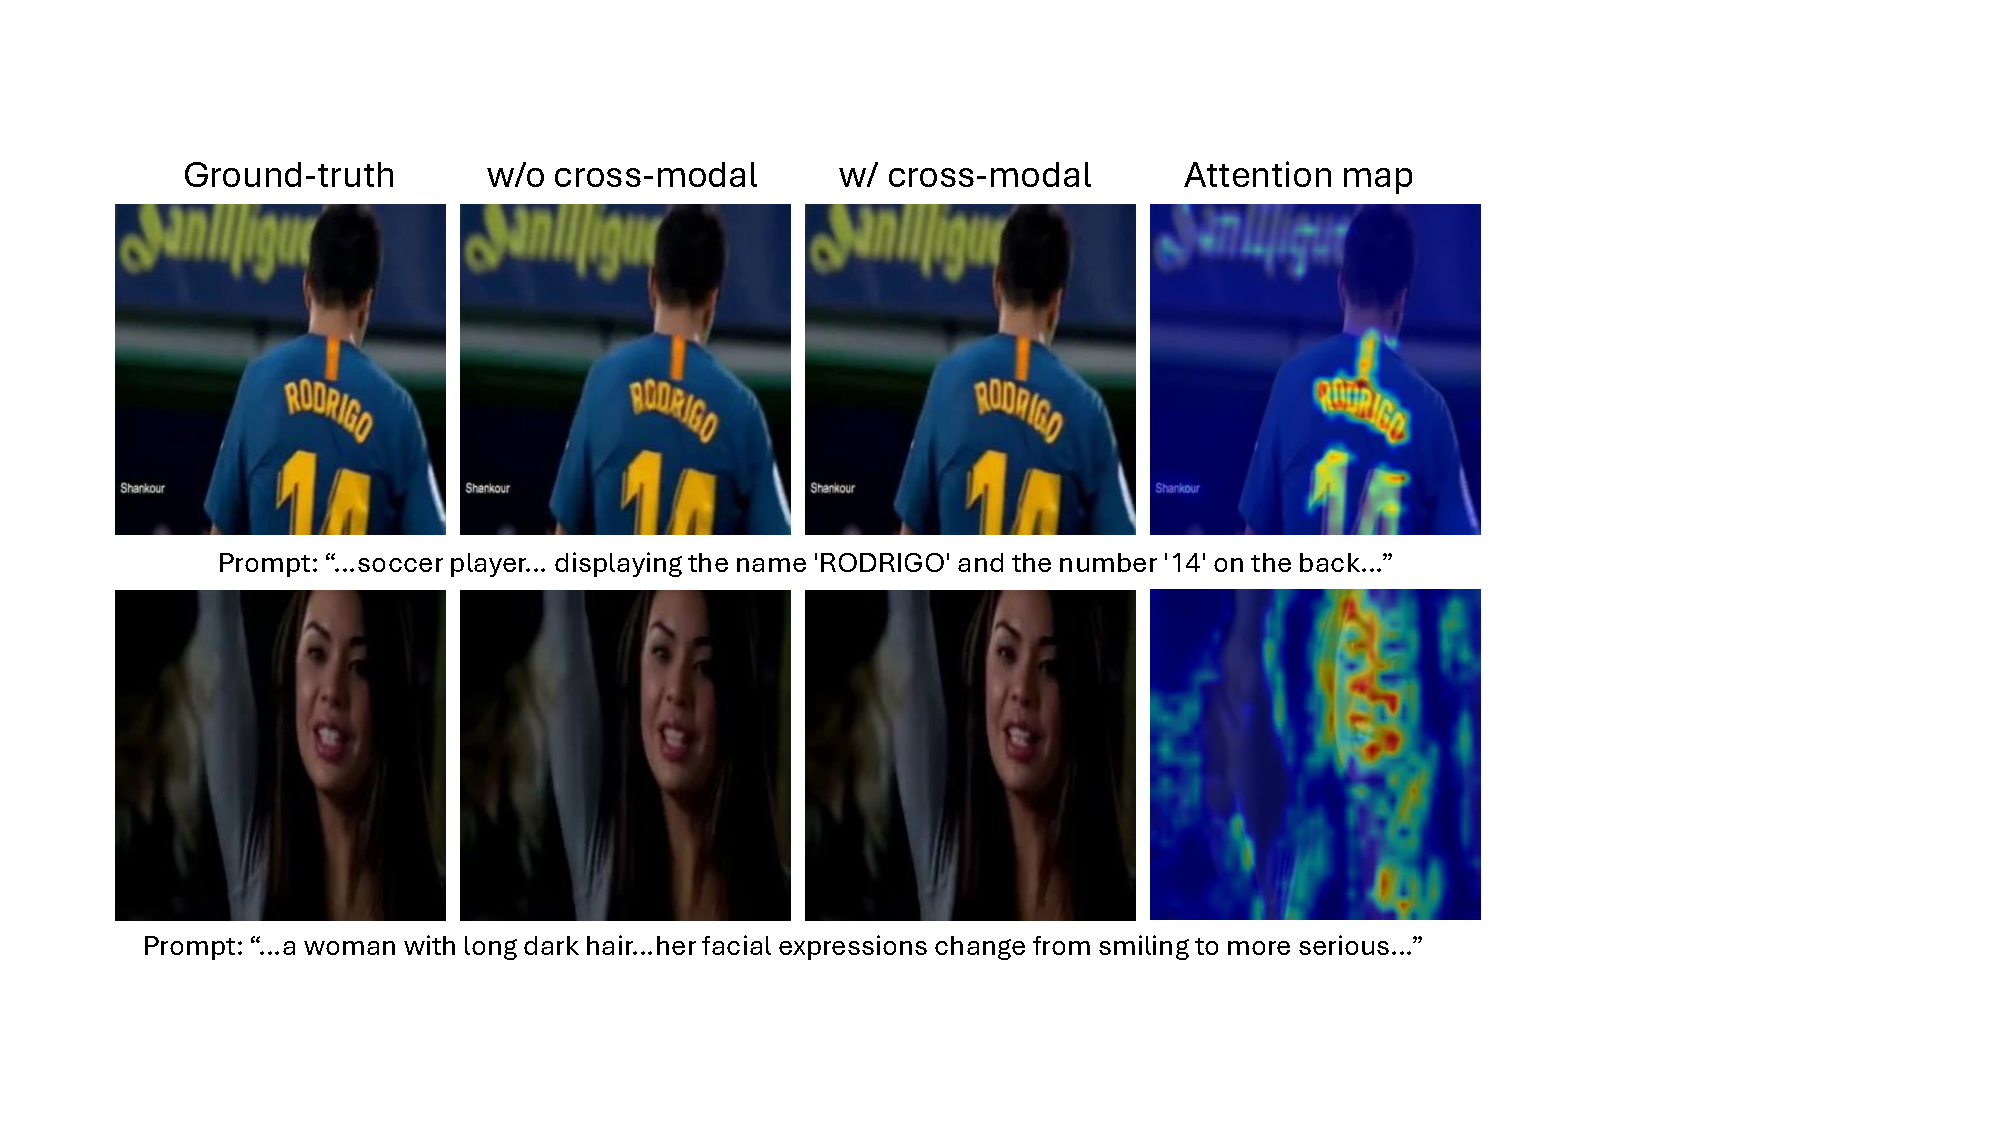
\includegraphics[width=0.48\textwidth]{images/crossattn.pdf}
\caption{The effectiveness of the cross-modal learning for our video VAE. The introduction of textural information improves the detail recovery. We visualize the learned attention map using keywords of the input prompts. 
}
\label{fig:cross}
\vspace{-3mm}
\end{figure}

\paragraph{Joint Training}
We evaluate the effectiveness of our image-video joint training by comparing the performance of our 4-channel latent and 16-channel latent Video VAEs with the video-only training VAE, as well as the image VAE,  SD 1.4 and SD 3.5, respectively. The results are shown in Table~\ref{tab:main} and Table~\ref{tab:ablation_joint}. The video reconstruction comparison is conducted on the three benchmark datasets. The image reconstruction comparison is conducted on a set of 500 images with a resolution of 480x864, randomly sampled from a UHD-4K video dataset. 
During inference, we mask out the temporal autoencoder and the temporal part of the temporal-aware spatial autoencoder, ensuring that the models process the images without considering temporal information, effectively treating them as independent images.

The joint training can further boost the performance of video reconstruction, which is consistent in both the 4-channel and 16-channel experiments. 
For the image reconstruction, our 4-channel latent Video VAE slightly outperforms SD1.4, and also improves on SSIM and LPIPS, indicating better perceptual quality.

For the 16-channel VAE, while our model achieves competitive results in terms of PSNR, it falls slightly short of SD3.5. However, our model still demonstrates strong performance in terms of SSIM and LPIPS, suggesting that our joint training approach maintains high perceptual quality despite the slight drop in PSNR.

We further show the visual effectiveness of the joint image and video training in Fig~\ref{fig:joint}. Overall, these results demonstrate that our joint image-video training strategy allows the model to retain strong image reconstruction capabilities while simultaneously learning to handle video data.

\begin{figure}[t]
\centering
\includegraphics[width=0.5\textwidth]{images/joint_result.pdf}
\caption{The effectiveness of joint image and video training.   
}
\label{fig:joint}
\vspace{-5mm}
\end{figure}


\begin{table}[ht]
    \centering
    \setlength\tabcolsep{2pt} % Adjusted column separation for better spacing
    \renewcommand{\arraystretch}{1.2} % Adjusted row height for readability
    \begin{tabular}{lcccc}
        \toprule
        \textbf{Model} & \textbf{PSNR ($\uparrow$)} & \textbf{SSIM ($\uparrow$)} & \textbf{LPIPS ($\downarrow$)} \\
        \midrule 
        \textbf{Simultaneous } & \underline{24.0593} & \textbf{0.7315} & \underline{0.1293} \\
        \textbf{Sequential} & 23.3681 & 0.6917 & 0.1481 \\
        \textbf{Ours} & \textbf{24.6722} & \underline{0.7234} & \textbf{0.1162} \\
        \bottomrule
    \end{tabular}
    \caption{Ablation study comparing simultaneous modeling, sequential modeling, and ours on the large-motion test set.}
    \label{tab:ablation_architecture}
    \vspace{-5mm}
\end{table}


\paragraph{Architecture Variants}
We evaluate the effectiveness of different spatiotemporal compression strategies, including simultaneous spatiotemporal compression, sequential spatiotemporal compression, and our proposed solution. These architecture variants are tested on the Large-Motion Test Set to determine which model handles challenging scenarios most effectively, as shown in Table~\ref{tab:ablation_architecture}. 

\begin{table}[ht]
    \centering
    \setlength\tabcolsep{2pt} % Adjusted column separation for better spacing
    \renewcommand{\arraystretch}{1} % Adjusted row height for readability
    \begin{tabular}{lcccc}
        \toprule
        \textbf{Model / Kernel Size} & \textbf{PSNR ($\uparrow$)} & \textbf{SSIM ($\uparrow$)} & \textbf{LPIPS ($\downarrow$)}  \\
        \midrule
        \textbf{Image GAN Loss} &  \underline{31.9133} & \underline{0.9071} & \underline{0.0436}  \\
        \textbf{Video GAN Loss} & \textbf{32.0262} & \textbf{0.9089} & \textbf{0.0426} \\
        \midrule
        \textbf{TemporalConv(3, 1, 1)} & 30.3332 & 0.8898 & 0.0489 \\
        \textbf{TemporalConv(5, 1, 1)} & 30.8745 & 0.9004 & 0.0475  \\
        \textbf{TemporalConv(7, 1, 1)} & 31.2922 & \underline{0.9025} & 0.0458  \\
        \textbf{TemporalConv(5, 3, 3)} & \underline{31.3516} & 0.9011 & \underline{0.0437}  \\
        \textbf{TemporalConv(7, 3, 3)} & \textbf{31.7444} & \textbf{0.9074} & \textbf{0.0436}  \\
        \bottomrule
    \end{tabular}
    \caption{Ablation study comparing temporal-aware spatial autoencoder with image/video GAN loss, and different kernel sizes.}
    \label{tab:ablation_combined}
    \vspace{-5mm}
\end{table}



\paragraph{Component Ablation}
We perform ablation studies on several key components of our model. First, we investigate the impact of the kernel size in the temporal convolutional layer of temporal-aware spatial autoencoder. The results of this study are shown in Table \ref{tab:ablation_combined}. Additionally, we explore the significance of the loss function by comparing the performance of temporal-aware spatial autoencoder trained with either the raw image GAN loss or the video GAN loss, with the results also presented in Table \ref{tab:ablation_combined}. These ablations are conducted on a validation set comprising 98 videos, each with a resolution of 256x256 pixels and a length of 16 frames, sourced from the MMTrailer dataset.









\vspace{-5pt}
\section{Conclusion}\label{sec:conclusion}
\vspace{-5pt}
We accelerate high-resolution diffusion models by designing deep compression autoencoders to reduce the number of tokens. We proposed two techniques: \textit{residual autoencoding} and \textit{decoupled high-resolution adaptation} to address the challenges brought by the high compression ratio. The resulting new autoencoder family \modelshort demonstrated satisfactory reconstruction accuracy with a spatial compression ratio of up to 128. \modelshort also demonstrated significant training and inference efficiency improvements when applied to latent diffusion models. 

\section*{Acknowledgements}
We thank NVIDIA for donating the DGX machines. We thank MIT-IBM Watson AI Lab, MIT and Amazon Science Hub, MIT AI Hardware Program, and National Science Foundation for supporting this research. 

{
    \small
    \bibliographystyle{ieeenat_fullname}
    \bibliography{main}
}

% WARNING: do not forget to delete the supplementary pages from your submission 
% \clearpage
\setcounter{page}{1}
\maketitlesupplementary


\section{Rationale}
\label{sec:rationale}
% 
Having the supplementary compiled together with the main paper means that:
% 
\begin{itemize}
\item The supplementary can back-reference sections of the main paper, for example, we can refer to \cref{sec:intro};
\item The main paper can forward reference sub-sections within the supplementary explicitly (e.g. referring to a particular experiment); 
\item When submitted to arXiv, the supplementary will already included at the end of the paper.
\end{itemize}
% 
To split the supplementary pages from the main paper, you can use \href{https://support.apple.com/en-ca/guide/preview/prvw11793/mac#:~:text=Delete%20a%20page%20from%20a,or%20choose%20Edit%20%3E%20Delete).}{Preview (on macOS)}, \href{https://www.adobe.com/acrobat/how-to/delete-pages-from-pdf.html#:~:text=Choose%20%E2%80%9CTools%E2%80%9D%20%3E%20%E2%80%9COrganize,or%20pages%20from%20the%20file.}{Adobe Acrobat} (on all OSs), as well as \href{https://superuser.com/questions/517986/is-it-possible-to-delete-some-pages-of-a-pdf-document}{command line tools}.

\end{document}
